The aforementioned approaches to define linked data lifecycles, see Section~\ref{sect:related-work}, are based on performing some processes, 
recipes, methods or tasks using different tools to promote raw data as RDF triples. However, a formal definition of processes, 
methods and tasks is missing and, in most of the cases, they are based on the author’s expertise. The main consequence 
of this offhand mixing of approaches is the lack of a quantifiable method to measure the quality of the generated RDF. 
That is why we have selected and applied the lifecycle proposed in the MOLDEAS project~\cite{DBLP:journals/ijseke/AlvarezLSASL12}
that perfectly defines which the steps to produce, publish, consume and validate linked open data are. Figure~\ref{fig:summary-tasks} summarizes several 
tasks to be carried out in order to promote a controlled vocabulary to the Linked Data effort. The formal definition of processes, 
methods and tasks in this lifecycle enables separation of concerns and the sustainable management of linked data. In the e-Government 
area this issue must be addressed due to the implicit responsibility of the public administrations of delivering high-quality services and data.

\begin{figure}[!ht]
\centering
	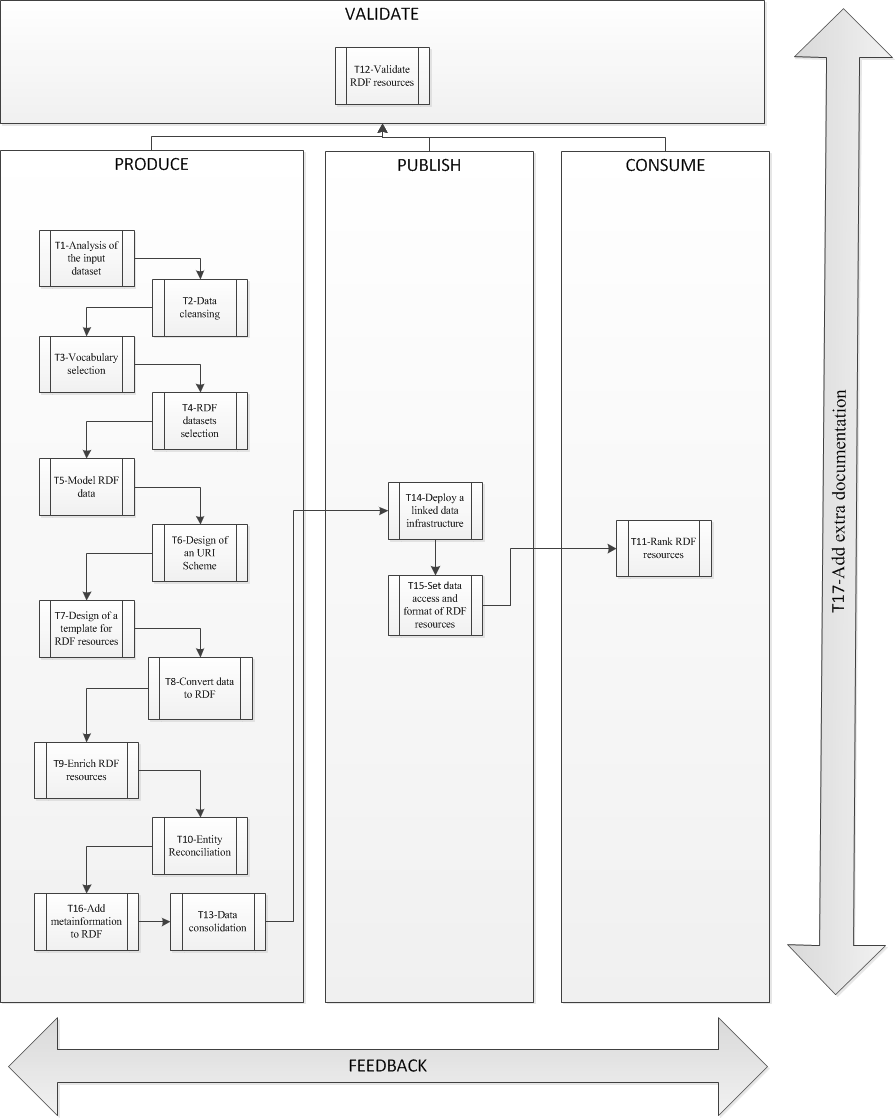
\includegraphics[width=\textwidth]{./imgs/fig-1}
 \caption{Summary of tasks of the MOLDEAS Linked Data lifecycle.}
 \label{fig:summary-tasks}
\end{figure}




